% Values: scripts/rq4_pacing_sizing_metrics.py, slack_profile() rows for
% 12MP normal (both devices pooled). Each bar is one 5% slack group [lo, lo+5);
% the light column behind it fills the group to 100%, so its visible part is
% the unpaced share. The line (right axis) is the median applied delay of the
% group's paced decisions, drawn only for groups with at least
% DELAY_MIN_PACED = 10 paced decisions (delayShown). Both axes start at zero.
% The plot shows slack 0-50%; the 1,053 decisions at or above 50% slack, of
% which 6 were paced, are stated in the RQ4 prose instead.
\begin{figure}[t]
  \centering
  \setlength{\abovecaptionskip}{2pt}%
  \setlength{\belowcaptionskip}{2pt}%
  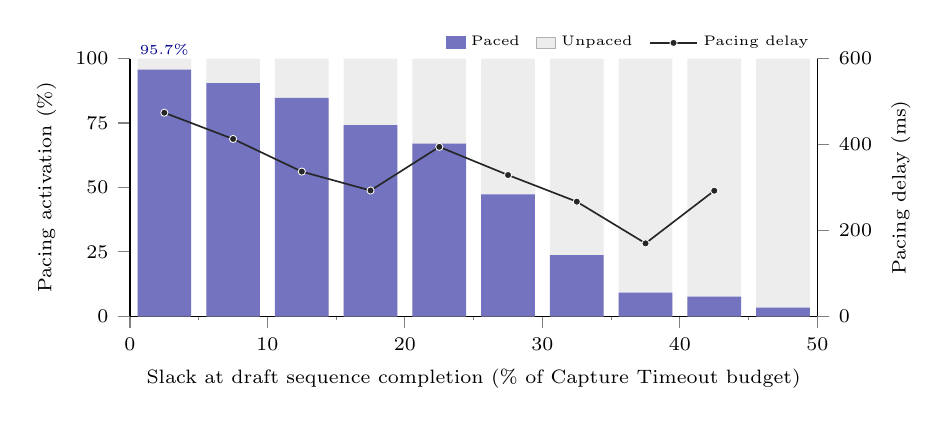
\begin{tikzpicture}
    \pgfplotsset{
      rq4 frame/.style={
        scale only axis=true,
        width=0.72\columnwidth,
        height=0.27\columnwidth,
        xmin=0,xmax=50,
        tick label style={font=\scriptsize},
        label style={font=\scriptsize},
        axis line style={line width=0.4pt},
        tick style={line width=0.4pt},
        tick align=outside,
        clip=false,
      },
    }
    \begin{axis}[
      rq4 frame,
      ybar,
      bar width=3.9,
      ymin=0,ymax=100,
      xtick={0,10,...,50},
      minor xtick={5,15,...,45},
      minor tick length=1.4pt,
      ytick={0,25,50,75,100},
      xlabel={Slack at draft sequence completion (\% of Capture Timeout budget)},
      ylabel={Pacing activation (\%)},
      axis x line*=bottom,
      axis y line*=left,
    ]
      \addplot[bar shift=0pt,draw=none,fill=black!7]
        coordinates {
          (2.5,100) (7.5,100) (12.5,100) (17.5,100) (22.5,100)
          (27.5,100) (32.5,100) (37.5,100) (42.5,100) (47.5,100)};
      \addplot[bar shift=0pt,draw=none,fill=blue!55!black!55]
        coordinates {
          (2.5,95.7) (7.5,90.5) (12.5,84.8) (17.5,74.2) (22.5,67.0)
          (27.5,47.3) (32.5,23.8) (37.5,9.2) (42.5,7.7) (47.5,3.4)};
      \node[anchor=south,font=\tiny,text=blue!55!black,inner sep=1pt]
        at (axis cs:2.5,100) {95.7\%};
    \end{axis}
    \begin{axis}[
      rq4 frame,
      ymin=0,ymax=600,
      ytick={0,200,400,600},
      ylabel={Pacing delay (ms)},
      axis y line*=right,
      axis x line=none,
      legend style={at={(1,1)},anchor=south east,font=\tiny,draw=none,
        fill=none,inner sep=1pt,legend columns=3,
        /tikz/every even column/.append style={column sep=4pt}},
      legend cell align=left,
    ]
      \addlegendimage{legend image code/.code={%
        \fill[blue!55!black!55]
          (0cm,-0.075cm) rectangle (0.24cm,0.075cm);}}
      \addlegendentry{Paced}
      \addlegendimage{legend image code/.code={%
        \draw[draw=black!30,fill=black!7,line width=0.2pt]
          (0cm,-0.075cm) rectangle (0.24cm,0.075cm);}}
      \addlegendentry{Unpaced}
      \addplot[black!85,line width=0.6pt,mark=*,mark size=1.3pt,
               mark options={fill=black!85,draw=white,line width=0.3pt}]
        coordinates {
          (2.5,474) (7.5,413) (12.5,337) (17.5,293) (22.5,394.5)
          (27.5,329) (32.5,267) (37.5,170) (42.5,292.5)};
      \addlegendentry{Pacing delay}
    \end{axis}
  \end{tikzpicture}
  \caption{Pacing activation and delay by slack (RQ4).}
  \label{fig:rq4_slack_activation}
\end{figure}
